\documentclass{beamer}

\usepackage{../../../latex_style/beamerthemeExecushares}
\usepackage{../../../latex_style/notations}

\title{Session 12: Gradient descent}
\subtitle{Optimization and Computational Linear Algebra for Data Science}
\author{Léo Miolane}
\date{}

\setcounter{showSlideNumbers}{1}

\begin{document}
\setcounter{showProgressBar}{0}
\setcounter{showSlideNumbers}{0}

\frame{\titlepage}
\setcounter{framenumber}{0}
%\setcounter{showProgressBar}{1}
\setcounter{showSlideNumbers}{1}

\begin{frame}
	\frametitle{Contents}
	\begin{enumerate}
		\item Gradient descent
		\item Convergence analysis for convex functions
		\item Improvements
	\end{enumerate}
\end{frame}

\section{Gradient descent}

\begin{frame}[t]{Gradient descent algorithm}
	\grid

	\vspace{-0.2cm}
	\textbf{Goal:} minimize a differentiable function $f: \R^n \to \R$.
	\vspace{-0.3cm}
	\begin{exampleblock}{}
		Starting from a point $x_0 \in \R^n$, perform the updates:
		$$
		x_{t+1} = x_t - \alpha_t \nabla f(x_t).
	\vspace{-0.2cm}
		$$
	\end{exampleblock}
	\hspace*{-5mm}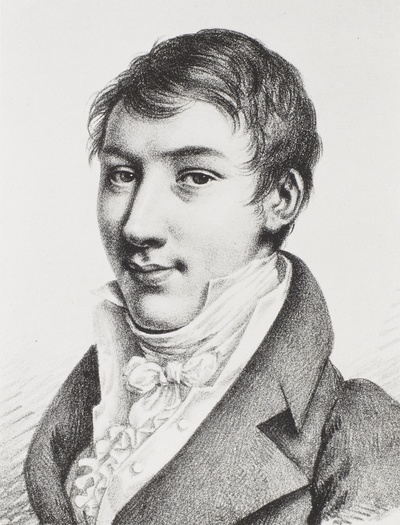
\includegraphics[width=3.5cm]{cauchy.jpg}

\end{frame}

\begin{frame}[t]{Convex  \ \ vs \ \ non-convex}
	\grid

	\begin{columns}
		\begin{column}{0.45\textwidth}
			\begin{center}
				\textbf{Convex}
			\end{center}
			\vspace{7cm}
	\end{column}
	\vrule
		\begin{column}{0.55\textwidth}
			\begin{center}
				\textbf{Non-convex}
			\end{center}
			\vspace{7cm}
	\end{column}
	\end{columns}

\end{frame}

\begin{frame}[t]{Numerical observations}
	\grid

	\begin{itemize}
		\item If the step size $\alpha$ is small enough, gradient descent converges to $x^{\star}$ \textbf{but} this may take a while.
			\vspace{0.4cm}
		\item If the step size $\alpha$ is large, gradient descent moves faster \textbf{but} it may oscilate or even diverge.
			\vspace{0.4cm}
		\item The convergence is faster when the eigenvalues of the Hessian $H_f$ are of close to each other.
	\end{itemize}

\end{frame}

\section{Convergence analysis for convex functions}

\begin{frame}[t]{Smoothness and strong convexity}
	\grid

	\vspace{-0.4cm}
	\begin{definition}
		Given $L,\mu > 0$, we say that a twice-differentiable convex function $f:\R^n \to \R$ is
		\begin{itemize}
			\item $L$-smooth if for all $x \in \R^n$, \ \ $\lambda_{\rm max}(H_f(x))\leq L$.
			\item $\mu$-strongly convex if for all $x \in \R^n$, \ \ $\lambda_{\rm min}(H_f(x))\geq \mu$.
		\end{itemize}
	\end{definition}
\end{frame}

\begin{frame}[t]{Speed for $L$-smooth functions}
	\grid

	\vspace{-0.4cm}
	\begin{block}{Proposition}
		Assume that $f$ is convex, $L$-smooth and admits a global minimizer $x^{\star} \in \R^n$.
		Then, gradient descent with constant step size $\alpha_t = 1/L$ verifies:
		$$
		f(x_t) - f(x^{\star}) \leq \frac{2 L \|x_0 - x^{\star}\|^2}{t+4}.
		$$
	\end{block}
\end{frame}

\begin{frame}[t]{$L$-smooth + $\mu$-strongly cvx functions}
	\grid

	\vspace{-0.4cm}
	\begin{block}{Theorem}
		Assume that $f$ is convex, $L$-smooth and $\mu$-strongly convex.
		Then, gradient descent with constant step size $\alpha_t = 1/L$ verifies:
		$$
		f(x_t) - f(x^{\star}) \leq \Big(1 - \frac{\mu}{L} \Big)^t (f(x_0) - f(x^{\star})).
		$$
	\end{block}
\end{frame}

\begin{frame}[t]{Proof}
	\grid

\end{frame}


\begin{frame}[t]{Choosing the step size}
	\grid

	\begin{block}{Backtracking line search}
		Start with $\alpha = 1$ and while
		$$
		f\big(x_t - \alpha \nabla f(x_t) \big) \geq f(x_t) - \frac{\alpha}{2} \|\nabla f(x_t) \|^2,
		$$
		update let's say $\alpha = 0.8 \alpha$.
	\end{block}
	\vspace{0.7cm}
	\hspace*{0.7cm}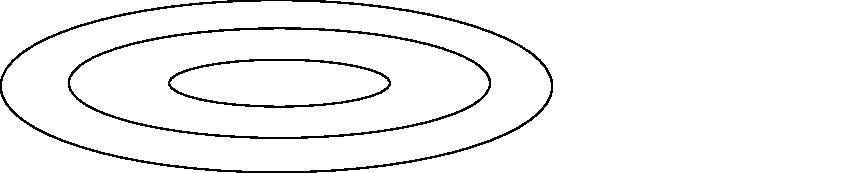
\includegraphics[width=15cm]{../figures/contour.pdf}
\end{frame}



\section{Improvements}


\begin{frame}[t]{Issues with gradient descent}
	\grid

	\vspace{-0.3cm}
	When the condition number $\kappa = L / \mu$ is large:
	\vspace{0.2cm}
	\begin{enumerate}
		\item the norm $ \|\nabla f(x) \|$ is sometimes too small.
			\below{\normalsize \color{ExecusharesRed} $\to$ gradient descent steps are too small.}
			\vspace{-1.0cm}$$
			$$
			\hspace*{1cm}
			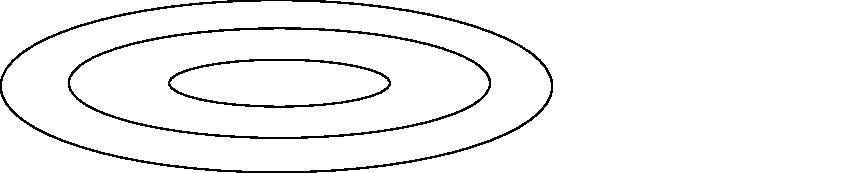
\includegraphics[width=11cm]{../figures/contour.pdf}
		\item The vector $- \nabla f(x)$ does << not really >> points towards the minimizer $x^{\star}$.
			\below{\normalsize \color{ExecusharesRed} $\to$ gradient descent oscilates.}
			\vspace{-1.0cm}$$
			$$
			\hspace*{1cm}
			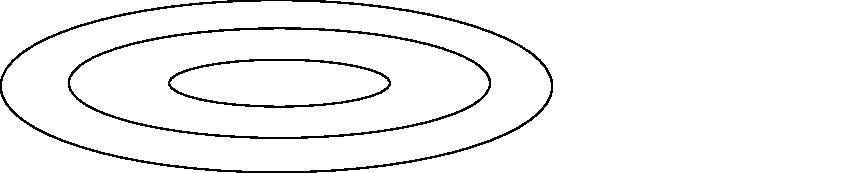
\includegraphics[width=11cm]{../figures/contour.pdf}
	\end{enumerate}

\end{frame}

\begin{frame}[t]{Gradient descent + momentum}
	\grid

	\textbf{Idea:} mimic the trajectory of an << heavy ball >> that goes down the slope:
	\vspace{-0.3cm}
	\begin{exampleblock}{}
		\vspace{-0.3cm}
		$$
		x_{t+1} = x_t + v_t \qquad \text{where} \quad v_t = - \alpha_t \nabla f(x_t)  \ + \ \beta_t v_{t-1} \,.
		$$
	\end{exampleblock}

	\vspace{0.7cm}
	\hspace*{0.7cm}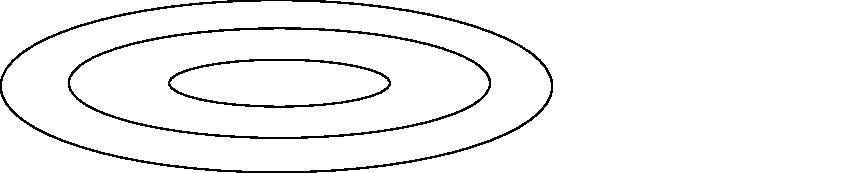
\includegraphics[width=15cm]{../figures/contour.pdf}
			

\end{frame}

\begin{frame}[t]{Newton's method}
	\grid

	\vspace{-0.2cm}
	Assume that $f$ is $\mu$-strongly convex and $L$-smooth.
		\vspace{-0.3cm}
	\begin{exampleblock}{}
		Newton's method perform the updates:
		$$
		x_{t+1} = x_t - H_f(x_t)^{-1} \nabla f(x_t).
		$$
	\end{exampleblock}
\end{frame}

\begin{frame}[t]{Graphical interpretation}
	\grid


\end{frame}

\begin{frame}[t]{Advantages and drawbacks}
	\grid

			\vspace{-0.2cm}
	\begin{itemize}
		\item Extremly fast there exists $C,\rho > 0$ such that
			$$
			\|x_t - x^{\star} \|^{2} \leq C e^{- \rho 2^t}.
			$$
		\item Computationally expensive: requires $\sim n^3$ operations to compute the inverse of the $n \times n$ matrix $H_f(x_t)$.
			\vspace{0.2cm}
		\item In non-convex setting, Newton's method gets attracted by any critical points (which could be saddle points/maximas...).
	\end{itemize}

			\vspace{0.5cm}
	\textbf{Quasi-Newton methods}: try to approximate $H_f(x_t)$ by matrices $B_t$ that are easier to compute.

\end{frame}


\appendix
\backupbegin
\begin{frame}[t]
	\frametitle{Questions?}
	\grid

	\pause
\end{frame}
\backupend




\end{document}
